%------------------------------------------------------------------------------
% Sablona dokumentu pro projekt predmetu PDS
% Autor: Petr Pospichal (xpospi45)
% Upravil: Jaroslav Dytrych (xdytry00), Petr Zemek (xzemek02)
%------------------------------------------------------------------------------
%==============================================================================
% Nazev projektu: Serial-TCP/IP bridge
% Autor: Petr Zemek, xzemek02@stud.fit.vutbr.cz
% Datum: 6.3.2009
%==============================================================================

\section{Introduction}

Regardless of the lack of the serial port \cite{WikiSerialPort} on most of the
current computers for masses, it is still useful -- mostly because of its
simplicity. For example, it is used to update firmware on various consumer devices,
for microcontrollers programming and connecting various devices like mice, printers and modems
to a computer. It is also used for network devices configuration, like routers.

One typically communicates with the serial device directly through the serial port
via a locally installed computer terminal emulator, which has the disadvantage
that one has to be physically working with the terminal. But what if one needs
to configure some router remotely from the Internet? This is the situation
where the serial-TCP/IP bridge comes handy.

\begin{figure}[ht!]
	\begin{center}
		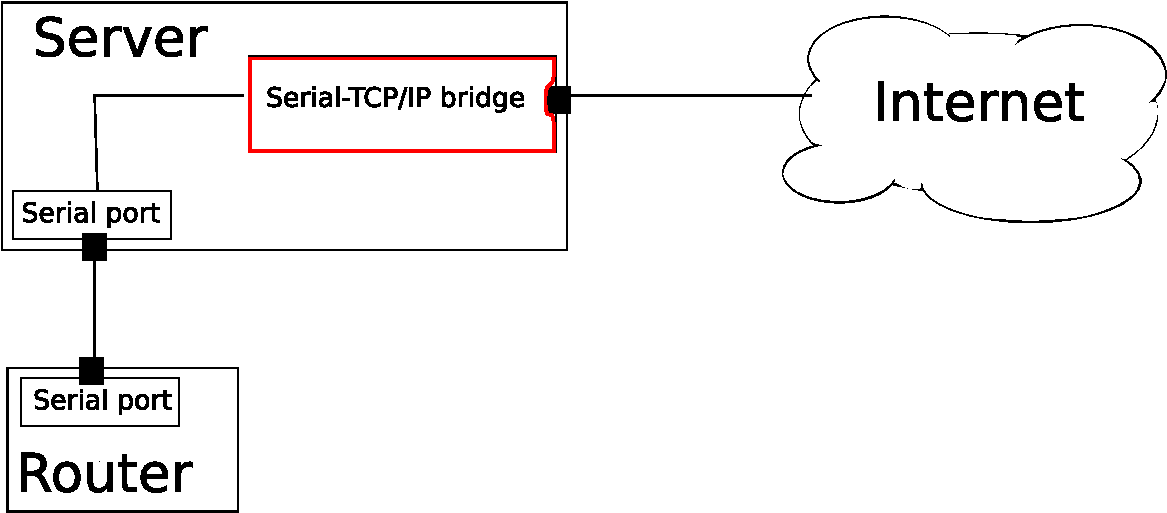
\includegraphics[width=8cm,keepaspectratio]{introduction}
		\caption{The role and position of the serial-TCP/IP bridge.}
		\label{serial-tcpip-bridge-role}
	\end{center}
\end{figure}

Figure \ref{serial-tcpip-bridge-role} shows how it works. If there
is a server on which a serial-TCP/IP bridge is running, one can connect
to that bridge via \texttt{telnet} or \texttt{netcat} from the Internet and
communicate with the serial device remotely. The bridge resends everything
from the client to the serial port and when there is a message from the serial
device, it resends it to the client.

The following sections describe design and implementation of such a serial-TCP/IP bridge.
Program usage is also included.

\section{Project design}

This section describes the project design. First there is an overall view
on the classes used in the project, then the concurrent behaviour of the server
is discussed and finally the way how errors are handled is given.

\subsection{Overall design}

\begin{figure}[ht!]
	\begin{center}
		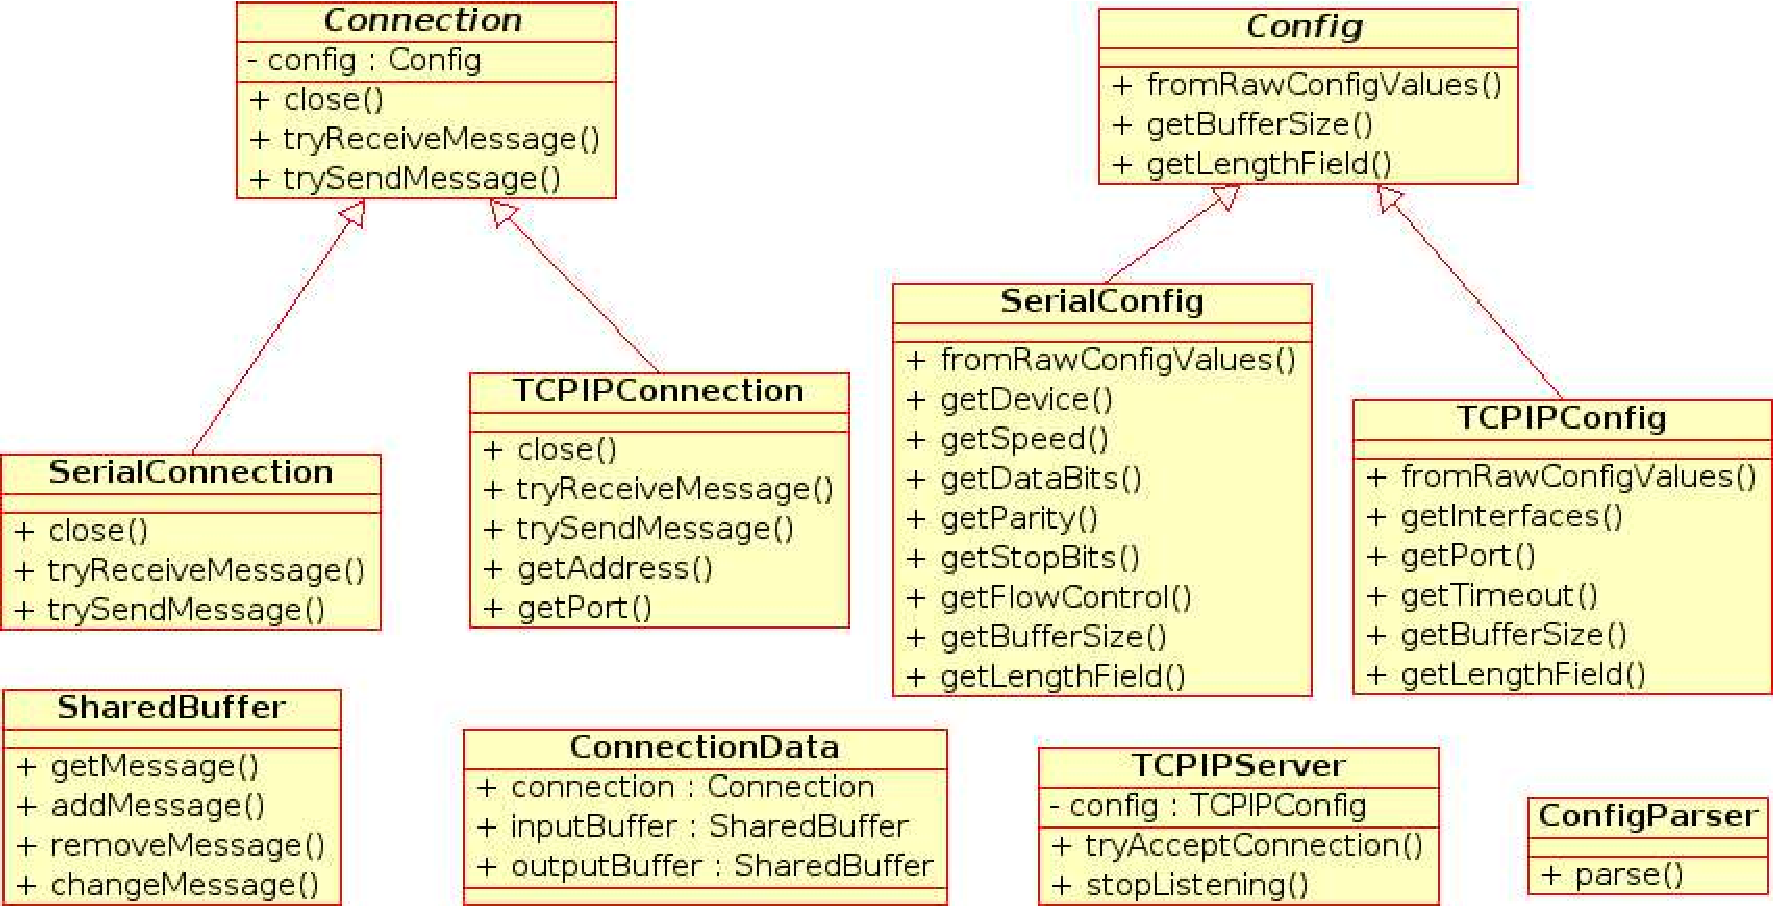
\includegraphics[width=14cm,keepaspectratio]{overall-class-diagram}
		\caption{Overall class diagram.}
		\label{overall-class-diagram}
	\end{center}
\end{figure}

Figure \ref{overall-class-diagram} shows the overall class diagram.
The \texttt{ConfigParser} class is used to parse a bridge configuration file into
an object (see the implementation part) which is then used to create instances
of two configuration classes:
the \texttt{SerialConfig}, which is used to setup the serial port and the \texttt{TCPIPConfig},
which is used to configure the TCP/IP part of the bridge. This part is represented
by the \texttt{TCPIPServer} class, which accepts client connections to the bridge,
which are represented by the \texttt{TCPIPConnection} class.
The \texttt{ConnectionData} class is used to store a connection (along with
other information) with input and output buffer, which are represented by
the \texttt{SharedBuffer} class.

\subsection{Concurrent server behaviour}
\label{ConcurrentServerBehaviour}

\begin{figure}[ht!]
	\begin{center}
		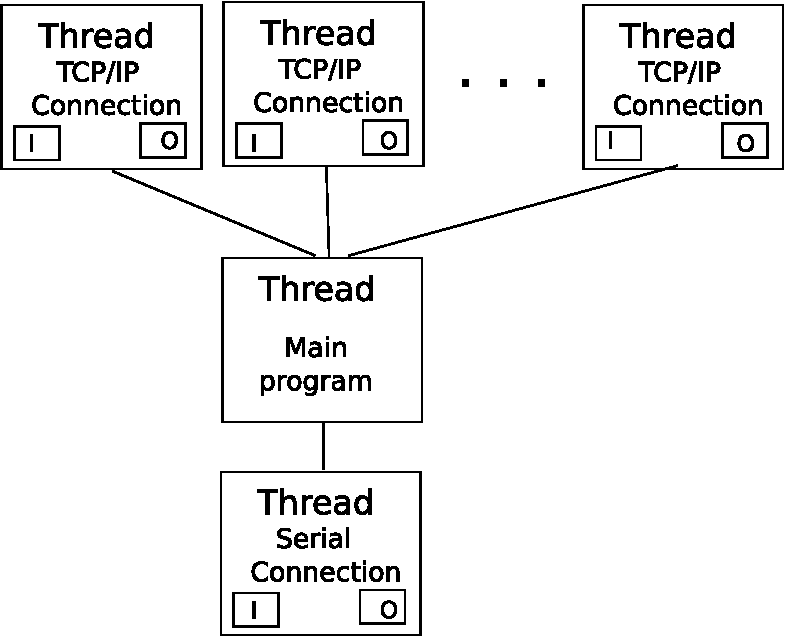
\includegraphics[width=5cm,keepaspectratio]{concurrency}
		\caption{How the concurrent behaviour is achieved.}
		\label{concurrency}
	\end{center}
\end{figure}

One part of the assignment was that the bridge must be concurrent,
i.e. it has to be able to serve more than one client at a time. To achieve this,
I decided to implement a threaded bridge, so it has a main thread which accepts
client connections and creates one thread per connection.
Figure \ref{concurrency} depicts this kind of a solution.

Note that there is also a separate thread for the communication with the serial
port. The main thread also transfers messages between connection buffers,
so when there is a message in the serial connection output buffer, it
copies that message to each client connections input buffer. The same
actions are taken in case of a new message in a client connections output buffer
(the message is transferred to the serial connections input buffer).

% HACK
\pagebreak
\subsection{Error handling}

\begin{figure}[ht!]
	\begin{center}
		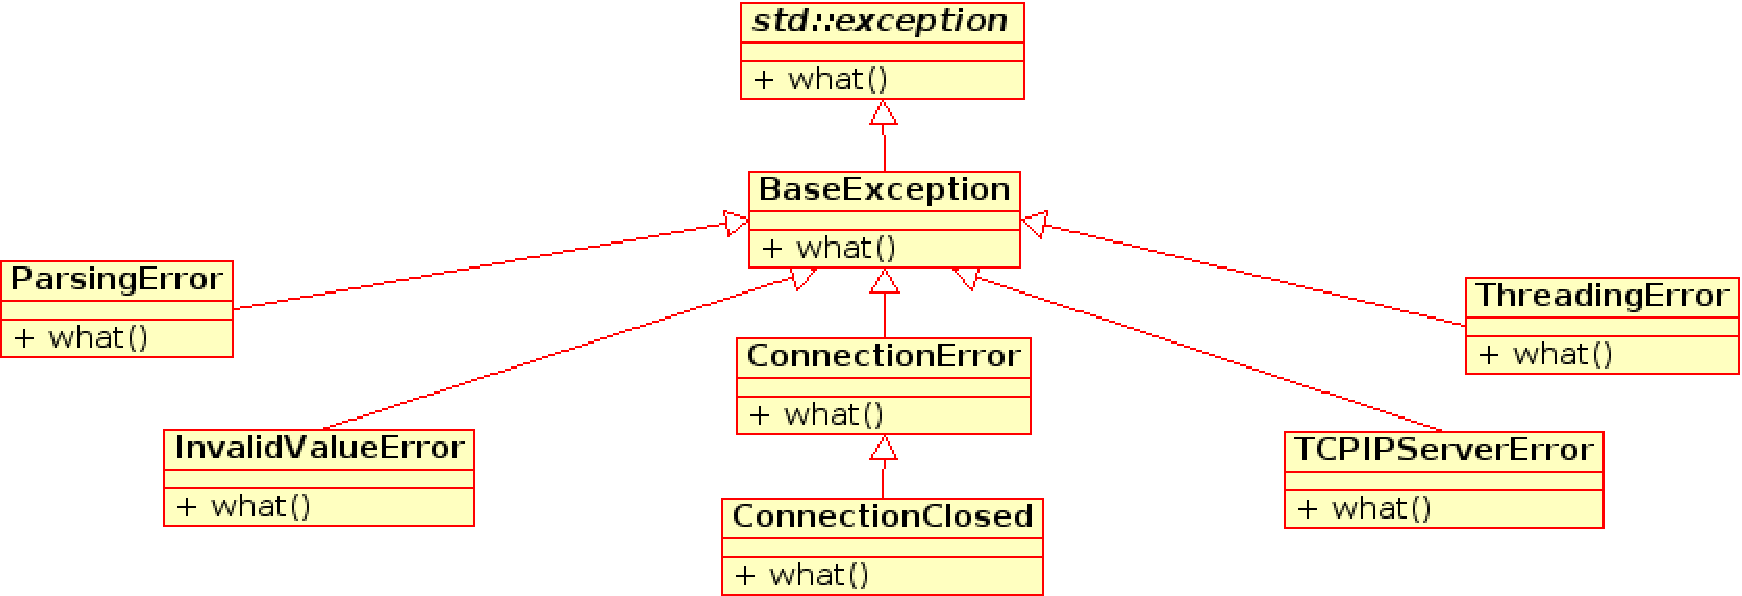
\includegraphics[width=14cm,keepaspectratio]{exceptions-class-diagram}
		\caption{Exceptions hierarchy.}
		\label{exceptions-class-diagram}
	\end{center}
\end{figure}

As for the error handling, I decided to use exceptions and I created a separate
exception for each area of problems (connection-related problems, threading
problems etc.).
Figure \ref{exceptions-class-diagram} shows the exception classes hierarchy in detail.

\section{Project implementation}

The bridge is implemented in C++ using the standard C library and C++98 library
(with STL) with GNU and POSIX extensions. The implementation details of all
project parts follows.

\subsection{Main program}

When the bridge is started, the passed configuration file is parsed
by the \texttt{ConfigParser} class. Since the grammar for the configuration file
is regular, I implemented it as a simple state machine. The parsed configuration
file is stored into an associative array (option name $\Rightarrow$ raw option value)
and this array is then used co create configurations for the serial part
and the TCP/IP part. Each configuration class (\texttt{SerialConfig} and
\texttt{TCPIPConfig}) gets from the array only options that are relevant to that
class purpose, parses them, checks their validity (there are several restrictions,
like the port number must be a natural number between $1$ and $65535$) and
stores them. If some option is missing, default values are used instead.

If both configurations are valid, instances of the \texttt{SerialConnection}
and \texttt{TCPIPServer} classes are created and the server starts accepting
connections. When there is a new connection, the server creates an instance of
the \texttt{TCPIPConnection} class and puts it into an instance of the
\texttt{ConnectionData} class, which is then stored into the connection data container.
The acceptance is nonblocking, so the bridge is also able to
transfer messages between buffer as was described in section \ref{ConcurrentServerBehaviour},
which is (apart from the connection acceptance part) the second most important
part of its job (it is fast so it does not cause any problems with new connections).

When there is an error or a request to stop the server (by sending a signal to
the bridge, like \texttt{SIGTERM}), it breaks the main loop, correctly ends
all connections and exits.

\subsection{TCP/IP part}

The TCP/IP part of the bridge (client connections acceptance, settings and
communication) is using UNIX sockets and was implemented according to
\cite{UNIXNetworkProgramming}.

To start listening and accepting connections, the \texttt{TCPIPServer} class uses
functions \texttt{socket()} and \texttt{fcntl()} (to create and setup a socket),
\texttt{setsockopt()} (to set port reusing),
\texttt{bind()} (to bind the address to the socket), \texttt{listen()} (to create
a client connection queue) and \texttt{accept()} (to accept an iccoming
client connection). The IP address of a network interface address is get
by using the \texttt{ioctl()} function. To make all operations nonblocking,
\texttt{fcntl()} is used.

The \texttt{TCPIPConnection} class uses functions \texttt{send()} and \texttt{recv()} to
send messages and receive them. Messages are stored into a buffer of a size
that is specified in the TCP/IP part of the configuration.

\subsubsection{Extensions, restrictions and things to note}

The configuration option \texttt{length\_field} can be maximally $4$ bytes,
because there are is no equivalent of the function \texttt{ntohl()}
for a number with more bytes than $4$.

Connection timeout is reseted not only when a message is received,
but also if a message is sent (to allow large data transfers).

\subsection{Serial part}

The serial part of the bridge (serial port settings and communication)
was implemented according to \cite{SerialHOWTO}, \cite{LinuxSerialPortProgramming}
and \cite{POSIXSerialProgramProgramming}.

The \texttt{SerialConnection} class uses functions \texttt{open()} (to open
the serial device), \texttt{tcgetattr()} and \texttt{tcsetattr()} (to set the
serial port). To make all operations nonblocking, \texttt{fcntl()} is again used.
Messages are received from the serial port by calling \texttt{read()}
and sent by calling \texttt{write()}.

\subsubsection{Extensions, restrictions and things to note}

Because there seems to be no way how to set $1.5$ stop bits on Linux, this
number of stop bits is \emph{not} supported. Mark and space parity is set using
an undocumented flag \texttt{CMSPAR} \cite{MarkSpaceParity}.

\subsection{Threading part}

As for the implementation of the threading behaviour, POSIX threads were used
and \cite{POSIXThreadsProgramming} was used as the main information resource.

After a connection is created (does not matter whether it is a TCP/IP
connection or a serial port connection), a handler (new thread) for that connection is
created using the \texttt{pthread\_create()} function. There is a loop in that
handler, in which the thread checks whether the connection should be closed
(expired connection timeout; uses \texttt{time()} to get the current time).
If so, then it closes that connection and signals to the main thread that this
connection should be removed from the connections container and exits.
After that, it checks whether there are is a message to be received and if so,
it receives it and put it into the output buffer. If there are any messages
in the input buffer, it sends the first one (only one message is sent in
a single loop pass).

Note that both buffers (input and output) can be accessed from the connection
handler and also from the main thread, so the operations on these buffers
have to be synchronized. To achieve this, functions \texttt{pthread\_mutex\_init()},
\texttt{pthread\_mutex\_lock()}, \texttt{pthread\_mutex\_unlock()} and
\texttt{pthread\_mutex\_destroy()} are used.
To ensure proper message removal from both buffers, messages are stored in
a pair (message, ID) and a message can be removed from the buffer by its ID.

\section{Program usage}

First you need to compile the program, so run \texttt{make} in the project
directory. After the compilation you can start the server by running:
\begin{center}
	\texttt{./bridge -f CONF\_FILE\_PATH}
\end{center}
where \texttt{CONF\_FILE\_PATH} is a configuration file path.
An example of the configuration file is provided in the project directory
(\texttt{bridge.cfg}).
The running server can be stopped by pressing \texttt{Ctrl+C} (when the server
is running on foreground) or sending a \texttt{SIGINT} or \texttt{SIGTERM} signal
(when the server is running on background) with \texttt{kill -SIGTERM `pidof bridge`}.

If the server was configured properly, you should be able to connect to it
by using \texttt{nc} (netcat; \texttt{nc interface port}) or simply
\texttt{telnet} (\texttt{telnet interface port}).

\section{Conclusion}

All specifications from the assignment were observed and satisfied during the
project development. Main parts were designed considering possible future
development and extensibility, like adding new configuration options, adding new
methods of data receiving or sending and lowering the CPU usage. The application
was successfully tested on the faculty server \texttt{merlin} (CentOS 5, 2.6.16,
x86-64) and on my two systems (Debian 5.0, 2.6.28, x86-64 and Kubuntu 8.04,
2.6.24, x86-32). Unit testing suites (63 tests in total) for some classes were
written using the \texttt{CPPUnit} library and run regularly. Memory leaks were
also taken into account and tested with \texttt{valgrind}
(\url{http://valgrind.org/}) and no memory leaks were discovered (even in case
of an error).

\subsection*{Used libraries}

Standard C library and C++98 library (with STL) with GNU and POSIX extensions \\
CPPUnit for unit testing (\url{http://cppunit.sourceforge.net/})

\subsection*{Metrices}

Source files: 35 \\
Source lines of code: 4029 (without empty lines) \\
Executable file size: 1.1 MB (GNU/Linux x86-64, g++ 4.3.2)
